\documentclass[12pt,a4paper]{article}
\usepackage[UTF8]{ctex}     %先引入ctex
\usepackage[utf8]{inputenc} %再引入inputenc
\usepackage{graphicx}
\usepackage{geometry}
\usepackage{xcolor}
% \usepackage{lazylatex}
\usepackage{amsmath}
\usepackage{enumerate}
\usepackage{caption}
\usepackage{listings}
\captionsetup[lstlisting]{labelfont=bf,justification=justified}

\usepackage{tikz}
\usepackage{pgfplots}
\pgfplotsset{compat=1.17}
\usepackage{appendix}

\graphicspath{{img/}}
% 边距
\geometry{left=2.0cm,right=2.0cm,top=2.0cm,bottom=3.0cm}
% 大题
\newenvironment{problems}{\begin{list}{}{\renewcommand{\makelabel}[1]{\textbf{##1}\hfil}}}{\end{list}}
% 小题
\newenvironment{steps}{\begin{list}{}{\renewcommand{\makelabel}[1]{##1.\hfil}}}{\end{list}}
% 答
\providecommand{\ans}{\textbf{答}:~}
% 解
\providecommand{\sol}{\textbf{解}.~}

\usepackage[colorlinks,linkcolor=blue]{hyperref}
\usepackage{bookmark}
\providecommand{\code}[2]{\lstinputlisting[language=#2,caption=\href{run:#1}{\ttfamily #1}]{#1}}
\providecommand{\img}[1]{\includegraphics[width=0.88\textwidth]{#1}}

% listings
\definecolor{grey}{rgb}{0.8,0.8,0.8}
\definecolor{darkgreen}{rgb}{0,0.3,0}
\definecolor{darkblue}{rgb}{0,0,0.3}
\lstset{%
    % numbers=left, %行号
    % numberstyle=\tiny\color{grey},
    showstringspaces=false,
    showspaces=false,%
    tabsize=4,%
    frame=shadowbox,%
    basicstyle={\ttfamily\scriptsize},%
    keywordstyle=\color{blue!80!black}\bfseries,%
    identifierstyle=,%
    commentstyle=\color{green!50!blue}\itshape,%
    stringstyle=\color{green!50!black},%
    rulesepcolor=\color{gray!20!white},
    breaklines,
    columns=flexible,
    extendedchars=false,
    %mathescape=true,
}

\begin{document}
\title{\normalsize \underline{操作系统(D)}\\\LARGE 项目 5}
\author{李子龙 518070910095}
\date{\today}
\maketitle

\begin{problems}
    \item[一] \textbf{设计线程池}

    开始时刻,输入5个线程,线程池处理这5个线程。

    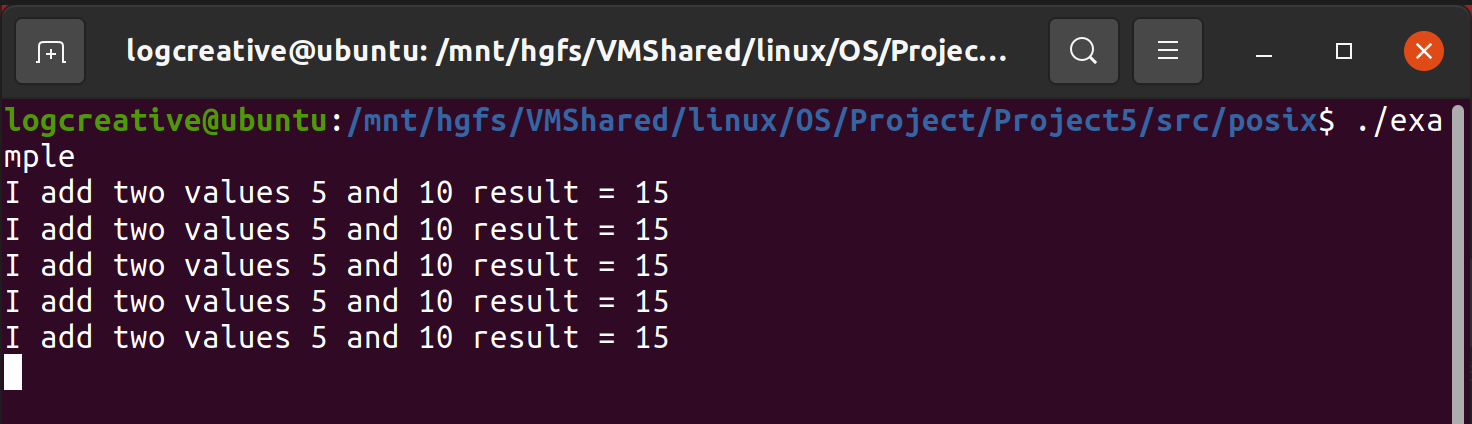
\includegraphics[width=0.88\textwidth]{threadpool1.png}

    后来,输入10个线程,但是线程池上限为9个线程,所以又只处理了9个线程。
    
    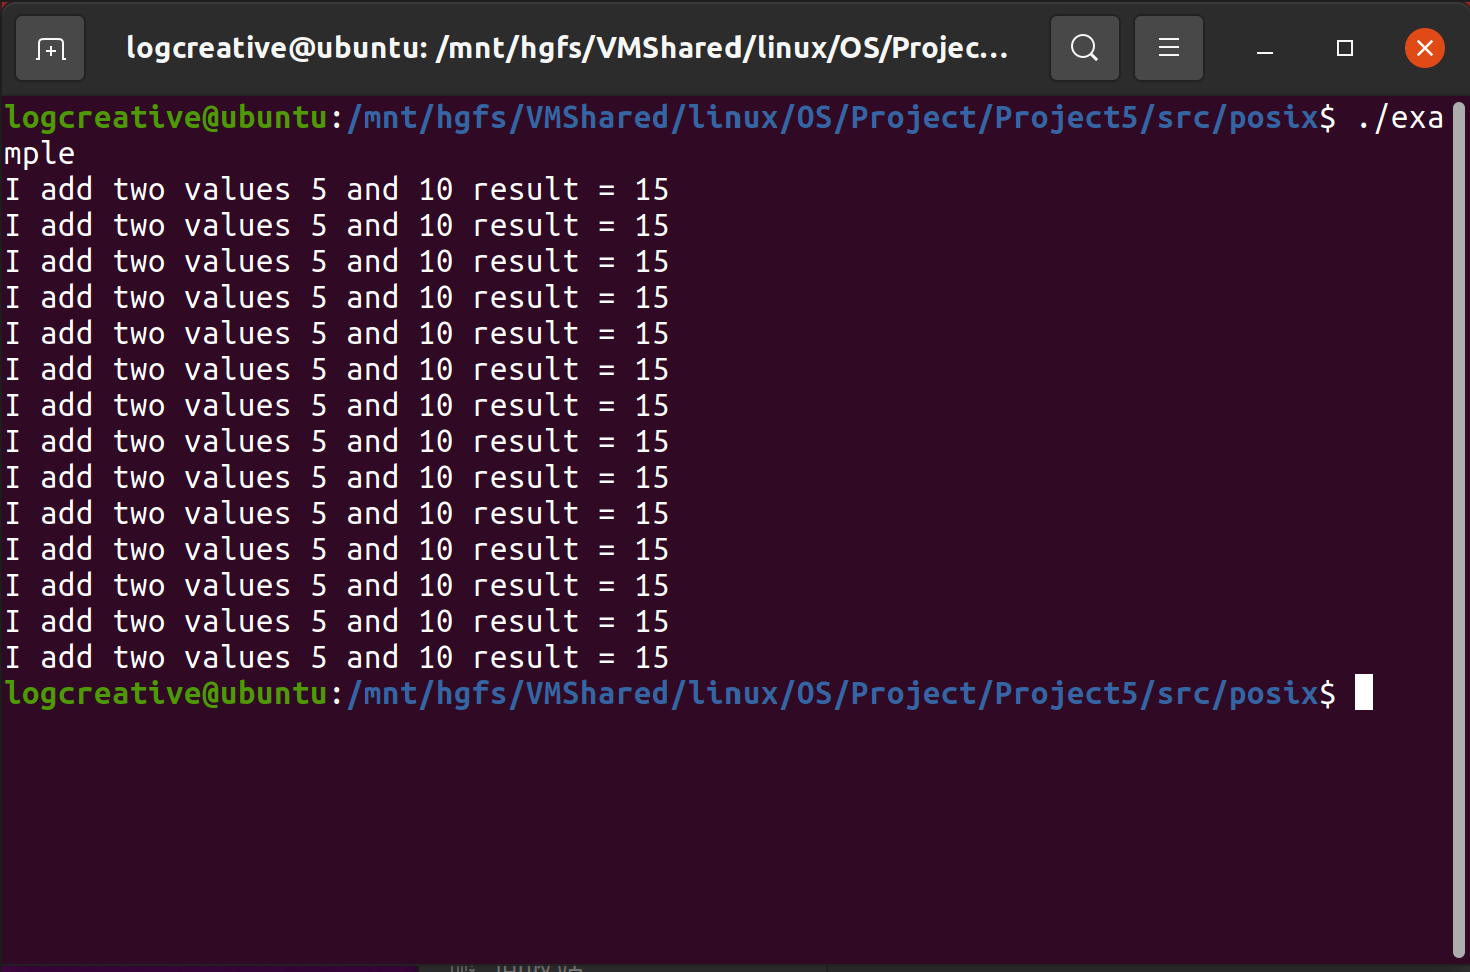
\includegraphics[width=0.88\textwidth]{threadpool2.png}

    \begin{steps}
        \item[1] \verb"pool_init()" 中初始化一个互斥锁和一个信号量。首先全局定义了两者后,再初始化 \verb"NUMBER_OF_THREADS = 3" 个 worker 线程。注意此处将 \verb"sem_submit" 初始化为 0。
        \begin{lstlisting}[language=c]
            // mutex
            pthread_mutex_t queue_mutex;

            // semaphore
            sem_t sem_submit;

            // initialize the thread pool
            void pool_init(void)
            {
                // mutual-exclusion locks
                pthread_mutex_init(&queue_mutex, NULL);
            
                // semaphores
                sem_init(&sem_submit, 0, 0);
            
                for(int i = 0; i < NUMBER_OF_THREADS; ++i)
                    pthread_create(&bee[i],NULL,worker,NULL);
            }
        \end{lstlisting}
        \item[2] \verb"pool_submit()" 需要使用队列存储任务。这里采用了循环队列。注意循环队列的容量是数据总量 - 1,也就是最多有 9 个任务可以在线程池中。
        \begin{lstlisting}[language=c]
            // the work queue
            task workqueue[QUEUE_SIZE];

            int front = 0, rear = 0;

            // insert a task into the queue
            // returns 0 if successful or 1 otherwise, 
            int enqueue(task t) 
            {

                pthread_mutex_lock(&queue_mutex);

                int res = 0;
                if((rear + 1) % QUEUE_SIZE == front) res = 1;
                else {
                    rear = (rear + 1) % QUEUE_SIZE;
                    workqueue[rear] = t;
                }

                pthread_mutex_unlock(&queue_mutex);
                
                return res;
            }

            // remove a task from the queue
            task dequeue() 
            {

                pthread_mutex_lock(&queue_mutex);

                front = (front + 1) % QUEUE_SIZE;
                task taskfront = workqueue[front];

                pthread_mutex_unlock(&queue_mutex);

                return taskfront;
            }
        \end{lstlisting} 
        \item[3] \verb"worker()" 进程,根据线程池的定义,一旦有可用进程就会从队列中弹出一个进程执行,并将需要服务的请求传递给它。一旦线程完成了服务,它会返回到池中再等待操作。如果池内没有可用线程,那么会等待,直到有空线程为止。这里使用一个信号量管理临界区入口。
        \begin{lstlisting}[language=c]
            // the worker thread in the thread pool
            void *worker(void *param)
            {
                while(TRUE){
                    sem_wait(&sem_submit);
                    // execute the task
                    task worktodo = dequeue();
                    execute(worktodo.function, worktodo.data);
                }

                pthread_exit(0);
            }
        \end{lstlisting} 
        \item[4] 为了防止对队列的同时操作,设置了相关互斥锁,在第 2. 点可见使用了 \verb"queue_mutex" 进行管理。
        \item[5] \verb"pool_shutdown()" 会首先对每一个线程进行线程撤销,最后进行线程合并。信号量是一个线程撤销点。
        \begin{lstlisting}[language=c]
            // shutdown the thread pool
            void pool_shutdown(void)
            {
                for(int i = 0; i < NUMBER_OF_THREADS; ++i)
                    pthread_cancel(bee[i]);
                for(int i = 0; i < NUMBER_OF_THREADS; ++i)
                    pthread_join(bee[i],NULL);
            }
        \end{lstlisting} 
    \end{steps}
    \item[二] \textbf{生产者--消费者问题}
    
    生产者比消费者多的情况:

    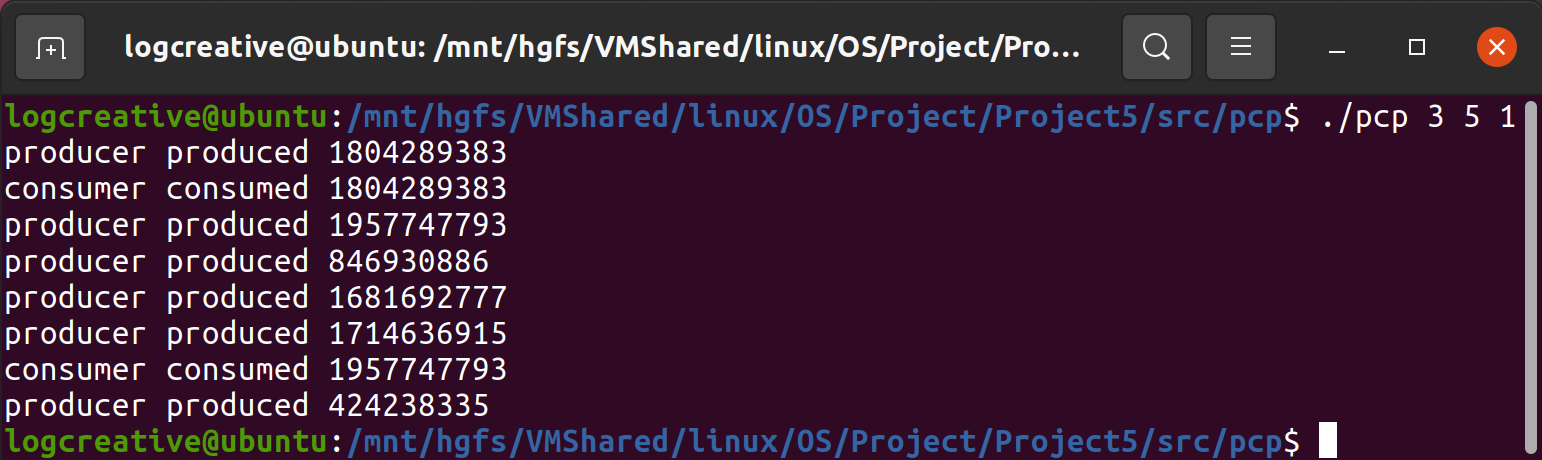
\includegraphics[width=0.8\textwidth]{pcpp.png}

    消费者比生产者多的情况:

    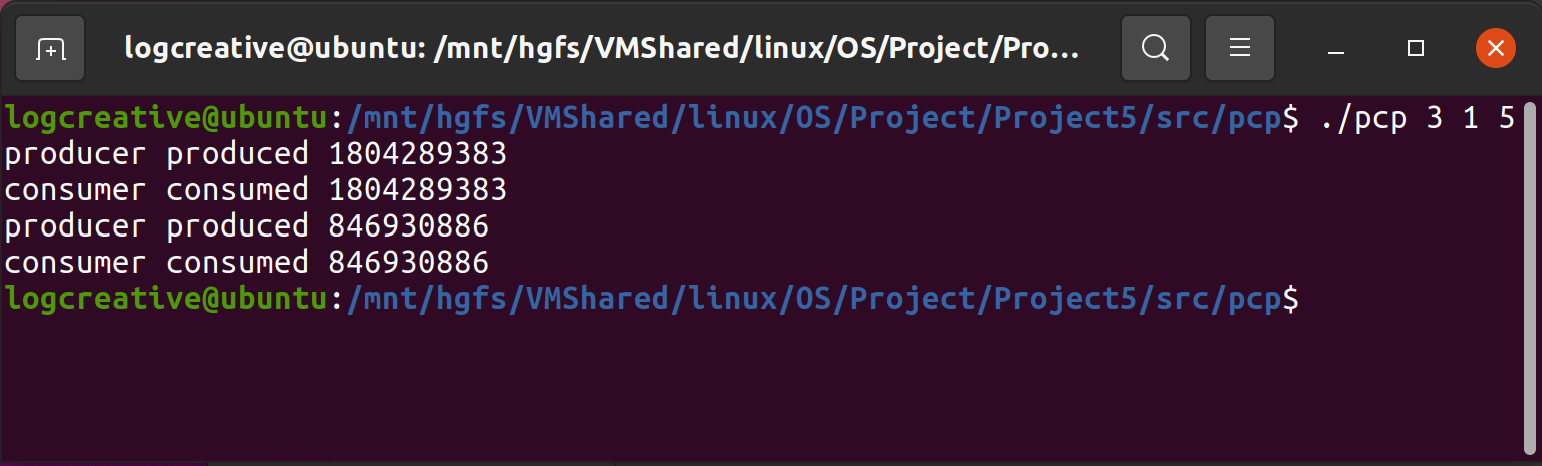
\includegraphics[width=0.8\textwidth]{pcpc.png}

    两个情况都没有报错,说明互斥锁与信号量运行正常。

    \begin{steps}
        \item[1] 缓冲区
        
        头文件定义如下:

        \code{src/pcp/buffer.h}{c}

        实现如下:

        \code{src/pcp/buffer.c}{c}

        这里使用了一个循环队列,同上一题。

        \item[2] 主函数。
        
        \begin{lstlisting}[language=c]
int main(int argc, char *argv[]){
    if(argc!=4){
        fprintf(stderr,"Three parameters are required!\n");
        return 1;
    }

    int sleep_amount = atoi(argv[1]);
    int p_count = atoi(argv[2]);
    int c_count = atoi(argv[3]);

    buffer_init();

    pthread_t* pbee = (pthread_t *) malloc(p_count*(sizeof(pthread_t)));
    for(int i = 0; i < p_count; ++i)
        pthread_create(&pbee[i], NULL, producer, NULL);
    
    pthread_t* cbee = (pthread_t *) malloc(c_count*(sizeof(pthread_t)));
    for(int j = 0; j < c_count; ++j)
        pthread_create(&cbee[j], NULL, consumer, NULL);
    
    sleep(sleep_amount);

    return 0;
}
        \end{lstlisting}

        按照要求的几点进行:
        \begin{enumerate}
            \item 获取相关参数。
            \item 初始化缓冲区。
            \item 创建生产者线程。
            \item 创建消费者线程。
            \item 主线程休眠以观察生产者与消费者的行为。
            \item 退出。
        \end{enumerate}

        \item[3] 缓冲区初始化函数。
        
        \begin{lstlisting}[language=c]
pthread_mutex_t mutex;
sem_t empty;
sem_t full;

void buffer_init(){
    pthread_mutex_init(&mutex,NULL);
    sem_init(&empty, 0, BUFFER_SIZE - 1);
    sem_init(&full, 0, 0);
}
        \end{lstlisting}

        定义了一个互斥锁,两个信号量。由于循环队列的容量是大小 - 1,所以 \verb"empty" 信号量被初始化为 \verb"BUFFER_SIZE - 1"。
        \item[4] 生产者函数。这里认为生产需要花费 1 秒。
        \begin{lstlisting}[language=c]
void *producer(void *param){
    buffer_item item;

    while(TRUE){
        sleep(1);
        item = rand();
        
        sem_wait(&empty);
        pthread_mutex_lock(&mutex);
        
        int error = 0;

        if(insert_item(item)){
            fprintf(stderr,"FULL!\n");
            error = 1;
        }
        else
            fprintf(stdout,"producer produced %d\n", item);

        pthread_mutex_unlock(&mutex);
        if(!error) sem_post(&full);
    }
}
        \end{lstlisting} 
        \item[5] 消费者函数。这里认为消费需要花费 1 秒。
        \begin{lstlisting}[language=c]
void *consumer(void *param){
    buffer_item item;

    while(TRUE){
        sem_wait(&full);
        pthread_mutex_lock(&mutex);
        
        int error = 0;
        if(remove_item(&item)){
            fprintf(stderr, "EMPTY!\n");
            error = 1;
        }
        else
            fprintf(stdout, "consumer consumed %d\n", item);

        pthread_mutex_unlock(&mutex);
        if(!error) sem_post(&empty);

        sleep(1);
    }
}
        \end{lstlisting} 
    \end{steps}
\end{problems}

\begin{appendices}
    \section{第一小项全部代码}
    \code{src/posix/threadpool.c}{c}
    \section{第二小项全部代码}
    \code{src/pcp/Makefile}{}
    \code{src/pcp/pcp.c}{c}
\end{appendices}

\end{document}
